% LTeX: language=en-GB
\chapter{Background and Research-Development Gap}
\label{chapter:SoA-and-RnD}

In technology development, it is important to gain a clear idea of two aspects:
\begin{enumerate}
    \item \textbf{Research aspect}: if the technology that is being developed requires the exploration of an uncharted research niche, as opposed to utilising pre-existing and consolidated knowledge for the creation of a new product;
    \item \textbf{Development aspect}: whether the proposed technology targets a well-defined market with unmet customer demand and no established supply.
\end{enumerate} 

This chapter explores both these aspects in Sections \ref{section:payload-first-approach}-\ref{section:airbag-design-variables} and \ref{section:market-analysis}, respectively. The aim is to gather sufficient background information, from market allocation of the proposed technology to concrete understanding of airbag design criteria, to depict the choices proposed in Chapter \ref{chapter:methodology} regarding operative \textit{methodology} as an answer to the Research Questions proposed at the end of this chapter.


\section{Regional Market Analysis: medical UAV logistics in Piedmont}\label{section:market-analysis}
The Italian National Healthcare System (\textit{SSN}) is structured hierarchically: the guidelines and regulations issued at a \textit{national} level must be implemented locally, at a \textit{regional} level, by each region's \textit{Sistema Sanitario Regionale} (\textit{SSR}, the Regional Healthcare Service). Vice versa, aviation rules follow European-level enforcement mechanisms: Following the 2019 harmonisation of European drone operations across the "open" and "specific" categories \cite{EU2019947}, operators seeking authorisation for high-risk flights are required to conduct a thorough risk analysis using the \textit{Specific Operations Risk Assessment (SORA)} methodology developed by JARUS\footnote{\textit{Joint Authorities for Rulemaking on Unmanned Systems}}, making a detailed evaluation of potential failure scenarios while proving compliance with the demanding safety standards imposed by aviation authorities. 

The discrepancy between modi operandi of the aviation and healthcare authorities has shaped the way drone-network operations have mostly been developing in the last decades in Italy: several emerging, albeit scattered, research groups, either cooperating or competing with industrial counterparts, have achieved geographically circumscribed trial deployments while being unable to scale the operation beyond testing.

A complete summary of such operations, limited to the means of investigation available for the present thesis project, can be found in Table \ref{tab:medical-drone-trials} in Appendix \ref{appendix:medical-drone-trials}. The table shows a clear trend: although potentially booming as several healthcare facilities are exploring the possibility of adopting drone transport and operators are proposing new drone models for them, most activities stop after the initial demonstrations, with the only exception being the region of Abruzzo where the operational phase of the drone drug-delivery service between a strategic hospital and village pharmacies was announced in July 2025 \cite{asl1_uelcome,abruzzospeciale_uelcome}. In general, a pattern of fragmentation, short-lived pilots, and few transitions to a potentially scalable service is observed in the construction of the overall \textit{value chain}, with many independent institutions covering equivalent roles, as shown in Table \ref{tab:actors} in Appendix \ref{appendix:value-chain-actors}.

 

{\longtablesetup
\begin{longtable}{G{0.14} L{0.17} L{0.27} L{0.42}}
\caption{Actors involved in drone delivery of medical goods in Piedmont, grouped by project.}
\label{tab:actors-piedmont}\\
\headrow\hd{Project} & \hd{Role} & \hd{Institution} & \hd{Scope} \\
\endfirsthead
\headrow\hd{Project} & \hd{Role} & \hd{Institution} & \hd{Scope} \\
\endhead
\contfoot{4}
\endfoot
\lastrule
\endlastfoot

% ---------------------------------------------------------------------
INDOOR (2021-2024)
& Promoter & Fondazione DOT & Project promoter \cite{dot_indoor} \\
\itemrule{3}
& Funder & Centro Nazionale Trapianti & Research grant at PIC4SeR \cite{dot_grant} \\
\itemrule{3}
& Funder & City of Turin & Project partner \cite{dot_indoor} \\
\itemrule{3}
& Research & PIC4SeR, Politecnico di Torino & Autonomous flight technologies for transporting biological material \cite{polito_pic4ser} \\
\itemrule{3}
& Research & Universit\`a di Torino & Project partner \cite{dot_indoor} \\
\itemrule{3}
& Technology partner & Mavtech & Technical partner; aerial surveillance and operational-support products \cite{dot_indoor} \\
\itemrule{3}
& Operator, payload maker & ABzero (Pisa) & Supplied the drone and the Smart Capsule (sensorised container for blood, organs and drugs); handled the ENAC authorisation \cite{abzero_web, cds_indoor, dot_grant, tecnomedicina_indoor} \\
\itemrule{3}
& End user & AOU Citt\`a della Salute e della Scienza & Test flight between hospital sites \cite{cds_indoor} \\
\itemrule{3}
& End user & Regional Transplant Centre Piemonte--Valle d'Aosta & Organ and biological transport \cite{dot_indoor} \\
\itemrule{3}
& Regulator & ENAC & National civil aviation authority; project partner and flight authorisation \cite{dot_indoor} \\
\grouprule
% ---------------------------------------------------------------------
DIMEAS feasibility studies (2020-2024)
& Research & DIMEAS, Politecnico di Torino (Prof.~E.~Cestino) & Desk-based feasibility studies for emergency drug delivery in Turin: regulatory platform selection and SORA, risk maps and path planning, payload thermal/vibration loads, cost--safety comparison of car, drone and eVTOL, hub siting \cite{Cavallo2020, Bertelli2021, Sivieri2021, Fiorentino2021, Angelini2023, Angelini2024ICAS} \\
\itemrule{3}
& Technology partner & FEV Italia & Industrial partner; numerical impact analysis \\
\itemrule{3}
& End user & AOU Citt\`a della Salute e della Scienza & Pharmacy department partner \\
\grouprule
% ---------------------------------------------------------------------
Hydrogen logistics plan
& End user & AOU Citt\`a della Salute e della Scienza & Proposed hydrogen drone logistics plan \cite{hydronews_torino} \\
\itemrule{3}
& Infrastructure & Torino Caselle and Cuneo Levaldigi airports & Proposed hub and support base \cite{hydronews_torino} \\
\grouprule
% ---------------------------------------------------------------------
LastMed
& Funder & City of Turin & Funded the LastMed call \cite{newpharma_lastmed} \\
\itemrule{3}
& Alternative (ground) & Tecnocad / Tecnomill / Bylogix & Autonomous ground rover for last-mile drug delivery \cite{ansa_lastmed} \\
\grouprule
% ---------------------------------------------------------------------
Independent
& Drone manufacturer & SkyEU & Autonomous high-speed eVTOL drones for first aid and critical logistics \cite{skyeu_web} \\
\itemrule{3}
& Regulator & Regione Piemonte & Regional health authority; drone trials subject to benefit--risk analysis \cite{cr_piemonte} \\
\end{longtable}
}

Adopting a region-based, rather than a nation-based, approach for market analysis is, therefore, necessary. Table \ref{tab:actors-piedmont} highlights stakeholders involved in Piedmont-based operations and their roles in the value chain, illustrating a fragmented scenario: Project INDOOR, launched by Fondazione DOT in 2021, culminated in a 500\,m-long test flight by an autonomous UAV between two Città della Salute hospital sites, carrying medical goods in a dedicated capsule, on 1st October 2024. In this project, several other stakeholders were involved (in fact, most of the ones present in Table \ref{tab:actors-piedmont}), among which ABzero (a spin-off from \textit{Scuola Normale Superiore di Pisa} responsible for capsule design and handling the ENAC authorisation process for the test flight), parallel research group PIC4SeR from the Department of Electronics and Telecommunications at \textit{Politecnico di Torino}, and \textit{MAVTech S.r.l.} (UAV systems designer company based in Turin). Independently of the INDOOR project of 2021-2024, the startup SkyEU was founded in 2025 promising to develop eVTOL drone systems for critical logistics within, but not limited to, the healthcare sector.

In parallel, and independently of INDOOR, the research group led by Prof. Enrico Cestino at the Department of Mechanical and Aerospace Engineering (DIMEAS) of \textit{Politecnico di Torino}, together with \textit{A.O.U. Città della Salute e della Scienza} and \textit{FEV Italia}, has pursued since 2020 a series of feasibility studies on the Molinette-San Giovanni Bosco route (Section \ref{section:prior-research}). These covered regulatory and mission evaluation, risk mapping and path planning, payload environmental loads, and cost-safety comparisons between road, drone and eVTOL transport. No flight campaign has been carried out so far. This makes the group the only Piedmontese actor whose work so far has been entirely at the planning and assessment level.

On the other hand, the regional administration's general stance with respect to this type of operation highlights the fundamental requirement of thorough benefit-risk analyses to guarantee both the safety of the Piedmontese citizens and the preservation of the medical cargo, possibly needing to limit transportation to exceptional emergencies in mountain areas \cite{cr_piemonte}. From an engineering perspective, these criticalities can be translated in the following barriers for the development of a full-scale, UAV-based delivery network:

\begin{enumerate}
    \item \textbf{Authorisation of flights}: Operations beyond the open category are approved by compiling the SORA. Among the different classes of mitigations, \textit{ground risk} mitigations (one of the first steps required in the SORA) reduce the consequences of the UAV's impact on the ground after a loss of control, for example by introducing a parachute. It is key for technical stakeholders to prove the reliability of their implemented ground risk mitigations to protect civilians in case of drone failure.
    \item \textbf{Payload integrity and containment}: In accordance with the regional administration's concerns, current certification standard UN3373 for ground handling of Biological Substances, Category B, establishes that packages must pass a drop test at 1.2\,m with no leakage from the primary container \hl{CITE STANDARD HERE, perhaps it needs a bit more detail}. However, in the event of a free-fall from ordinary mission altitudes, this standard loses its significance and the potential for biological material dispersion into the environment becomes highly relevant.  
    \item \textbf{Unsustainability of the current business models} While costs of road and helicopter transport of biomedical goods such as organs, drugs and other critical supplies are expected to fall significantly with drones, most trials are funded by EU projects and one-time grants, with the consequence of making the project unsustainable and non-scalable.
\end{enumerate}

On the basis of this analysis, several research and development gaps can be identified: SkyEU is endeavouring to enact an economically sustainable business model for large-scale UAV networks, but has a small public record; ABzero has patented capsules equipped with electronics that reliably monitor in-flight vibrations and guarantee thermal control of the medical payload, but these are only certified to the UN3373 standard, whereas in case of in-flight failure a much more conservative approach is needed; regional authorities need reassurance on the safety aspect for civilians, as a 500\,m test flight on a controlled route shows that the obstacle is not drone-making, but guaranteeing safety in everyday performance rather than in single monitored missions.

In this scenario, the institutions (\textit{Politecnico di Torino (DIMEAS), FEV Italia, AOU Città della Salute}) that commissioned the present thesis project aim to tackle, among the three barriers, barrier 2, concerning payload integrity and containment. The proposed solution is an airbag-type device that protects the payload and prevents its dispersion in the event of an impact, especially in view of transporting extremely valuable medicinals and/or biological materials, e.g. human organs for urgent transplant operations. This device is conceived as an add-on to existing capsules such as the one by ABzero or those mounted on drones such as SkyEU's (for which documented information remains unavailable at the time of writing), and is intended to help close the certification gap highlighted above, while acknowledging that it does not address the issues linked to SORA ground risk or the sustainability of the business model.



\section{\textit{Mission-first} vs. \textit{Safety-first}: a design-philosophy gap}\label{section:payload-first-approach}

This section builds on the research-development gap presented earlier by attempting to connect its root causes to a discrepancy between design philosophies applied in the aeronautical and the biomedical sectors. The proposed design solution (the airbag-type device) is, in fact, a suggestion to solve an "aeronautical problem" implementing a "medical approach".

The issue of proving compliance to match demanding safety standards imposed by the certification authorities does not appear to be a Piedmont-only (or even an Italy-only) problem, but rather a widespread trend that affects all non-standard aeronautical projects across the field. As highlighted, for example, in \cite{chhetri2026survey}, most UAV producers focus on optimising their aerial vehicle's design, minimising mission-related vibrational loads, thermal loads, overall mass, but also proposing ever more efficient cargo-drop mechanisms and ways to overcome geographical obstacles, all partaking in a feedback loop against aerodynamic and flight-mechanics performance metrics. This machine-centric approach appears to be the default, especially considering that UAV-based missions are, naturally, radically different from standard airline and/or general aviation operations, where passenger safety and vehicle safety are inherently aligned and where, therefore, stringent certification requirements strongly limit design freedom \hl{CITE ARTICLE HERE}. A common consequence of focusing exclusively on technological potential when designing UAV-based operations is, therefore, neglecting the safety assurance aspect of the project, which is usually delegated to including a parachute-type device in the final design phases. As pointed out by \cite{alulema2026how} in their design feasibility evaluation study, the introduction of a parachute usually increases the risk of falling into a mass-increase feedback loop: the parachute increases the airframe's overall mass, which then requires a larger, thus heavier, parachute for efficient deceleration during free-fall, which again results in an excessive mass increase, and so on. This negative feedback loop results either in never reaching design convergence, or otherwise in having to accept a smaller parachute with reduced deceleration capacity, still implying a relatively high ground-impact velocity and almost certainly destructive damage to the airframe, its cargo, and the impacted areas on the ground.     

The general impression given by the brief market analysis conducted earlier and the observations gathered in the present paragraph is that, perhaps, the "mission-first" approach adopted in the majority of nascent UAV-based operations is not sustainable for the projects' longevity beyond pilot flights, and that it might be necessary to embrace a paradigm shift in design approaches. Specifically, there might be potential in drawing inspiration from the biomedical field, where medical technology designers are encouraged to shift from a techno-centred to a human-centric approach to avoid the \textit{translation gap} or \textit{implementation gap}, i.e. the potential to introduce or enhance health inequity when trying to implement extremely advanced technology that does not take into account all necessities and limitations of human patients \cite{rodriguez2023thinking}. 

Just like success is measured on the patient and not on the device in the biomedical field, in the case of UAV-based medical delivery operations success should be measured on payload integrity and protection of civilians, not (only) on the capabilities of the aerial vehicle. A drone that survives an in-flight failure while sacrificing its payload and threatening irreversible human damage has undoubtedly failed its mission, as for a biomedical device that functions correctly but does not serve the patient. This reasoning leads to the first of the contributions proposed in the present thesis, which is the \textit{"safety-first"} design principle presented in Section \ref{section:outer-design-loop}. This thesis aims to serve as a test-bed for this proposed approach, where exploring the airbag design process helps bridge the gap between current development efforts and certification.


\section{Airbag impact attenuation: background knowledge}\label{section:airbag-design-variables}
Airbag-type devices have a well-established, enduring research-development record with contributions found across multiple industries. The information presented in Sections \ref{section:airbag-industry-perspective} and \ref{section:airbag-design-guidelines} aims to represent the State of the Art practices adopted in airbag design. The scope of this investigation is developing a solid, although perhaps not comprehensive, understanding of design recommendations on which to base the proposal for the design workflow of later Section \ref{section:inner-design-loop}.

\subsection{Established applications and common working principle}\label{section:airbag-industry-perspective}
Airbag technology is well established across two primary sectors: \textit{automotive} and \textit{aerospace}.

In the automotive industry, these systems are implemented during vehicle crashes, distinguishing between general automobile crashes and motorcycle impacts. In the space industry, ever since the early space missions of the 1960s, airbags have been deployed during the final landing phases of space capsules. Within the aeronautical industry, specifically in the "specific" operations category, other niche applications have emerged, such as the experimental study of adaptive airbag systems for the protection of UAVs and general aviation vehicles \cite{HolnickiSzulc2023} (following a long track record of exploration in the field of adaptive technologies for impact absorption \cite{HolnickiSzulc2015, HolnickiSzulc2009}). 

In either case, the primary objective of the airbag-type device remains the same: to be stored compactly in ordinary mission conditions, inflate within the allowable time before impact (whether during an emergency impact or landing), and decelerate the target body (whether a crash test dummy or a spacecraft) far more gently than in case of direct impact. When analysing these systems, purely analytical, hard-codable solutions are typically limited to single-degree-of-freedom (1-DoF) formulations, immediately resolving to the use of far more computationally-heavy finite element analyses to capture the complex two- and three-dimensional effects of the impact. The only exception to this trend is the technical report NATICK/TR-87/042 published by T. F. Patterson in 1985\footnote{T. F. Patterson, \textit{Design, Fabrication and Testing of an Airdrop Platform Utilizing Airbags as Shock Absorbers}, NATICK/TR-87/042, U.S. Army Natick Research, Development and Engineering Center, Aug. 1985.}, which presents a 6-DoF analytical simulation built on closed-form component models, but remains inaccessible at the time of writing of the present literature search.

Despite the diversity of fields, all applications share identical fundamental working principles. An example of an analytical study of airbag-based impact events, and one of the most significant papers in shaping this thesis' work, is Zhou et al. (2019) \cite{Zhou2019}, in turn heavily rooted in the SAND93-2133 technical report \cite{Cole1993} on a code for predicting the performance of the Pathfinder lander's airbag impact attenuation system, which describes the core working principle of airbag physics in a one-degree-of-freedom impact event. 

\begin{figure}[h]
    \centering
    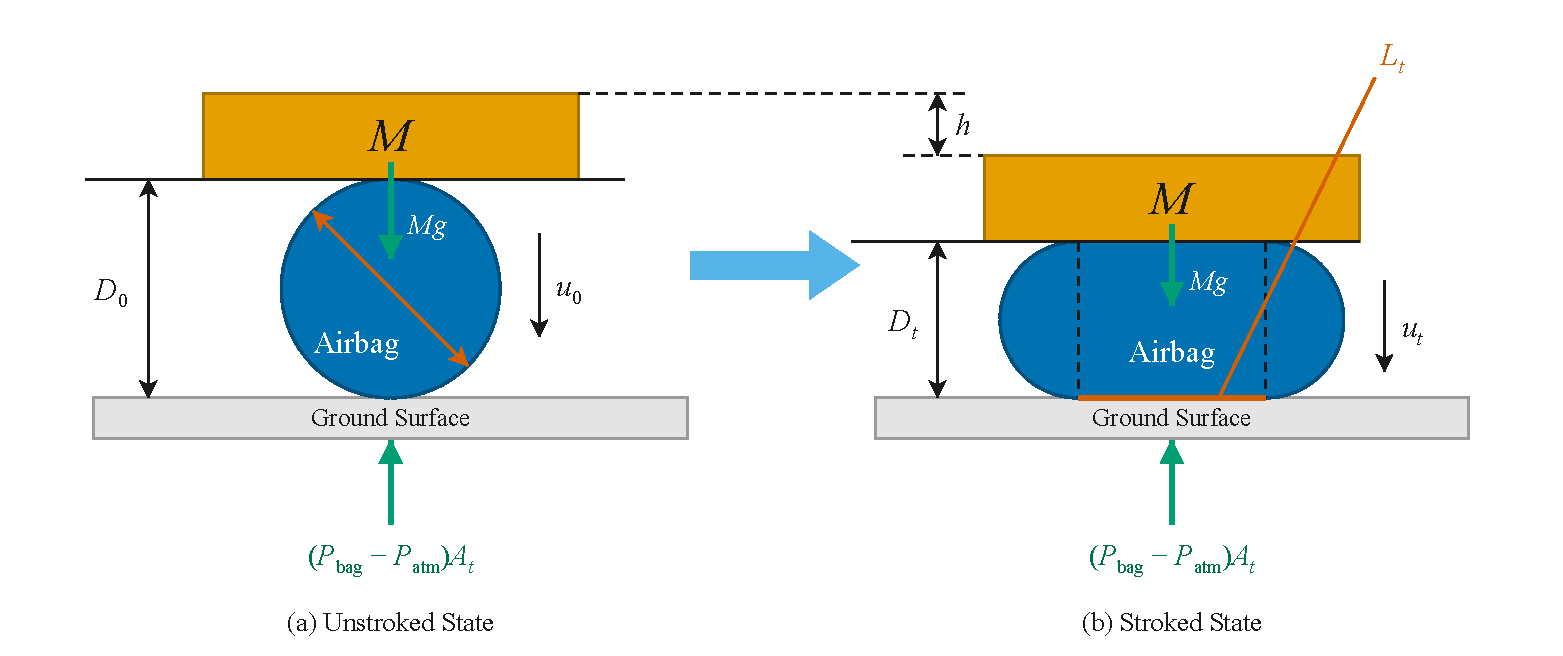
\includegraphics[width=\textwidth]{figures/chap2/Zhou-et-al_2019_diagram.pdf}
    \caption{One-degree-of-freedom airbag impact model in the unstroked (a) and stroked (b) states, adapted from Zhou et al. \cite{Zhou2019}.}
    \label{fig:zhou-airbag-1dof}
\end{figure}


The quantities under study for this type of phenomenon are shown in Fig.\ref{fig:zhou-airbag-1dof}, where a point load (yet, with a finite extension, as to avoid penetration in the airbag and justify the crude, though analytically necessary, \textit{uniform pressure/control volume} assumption, where pressure is uniformly distributed within the airbag volume) is protected by a single inflated airbag in incipient contact with the ground surface after a free fall. The quantities are:

\begin{itemize}
  \item $M$, the mass of the payload, which remains constant throughout the analysis and results in the vertically applied gravitational force $M g$.
  \item $u_0$, the initial impact velocity at time $t_0$, which evolves to $u_t$ after each subsequent time increment. It is updated at every time increment through kinematic analysis.
  \item $D_0$, the initial diameter of the airbag, which evolves to $D_t$ following the same loop update concept. Broadly speaking, its meaning can be extended to the characteristic dimension of the airbag, according to the airbag shape selected for the test case among the available options (vertically- or horizontally-oriented cylinder, sphere, toroid, etc.).
  \item $h$, the \textit{stroke}, i.e. the (vertical) distance covered by the payload when compressing the airbag during the impact event.
  \item $(P_{bag}-P_{atm})\cdot A_t$, the normal reaction force from the ground, based on the difference between the internal pressure of the airbag $P_{bag}$ and atmospheric pressure $P_{atm}$, multiplied by the footprint area $A_t$ with the ground, calculated according to different geometric assumptions correlating $A_t = f(h,t)$.

\end{itemize}

The reference system is downward-positive, in accordance with the direction of gravity and the initial velocity, making the reaction force negative.

\begin{figure}[h]
    \centering
    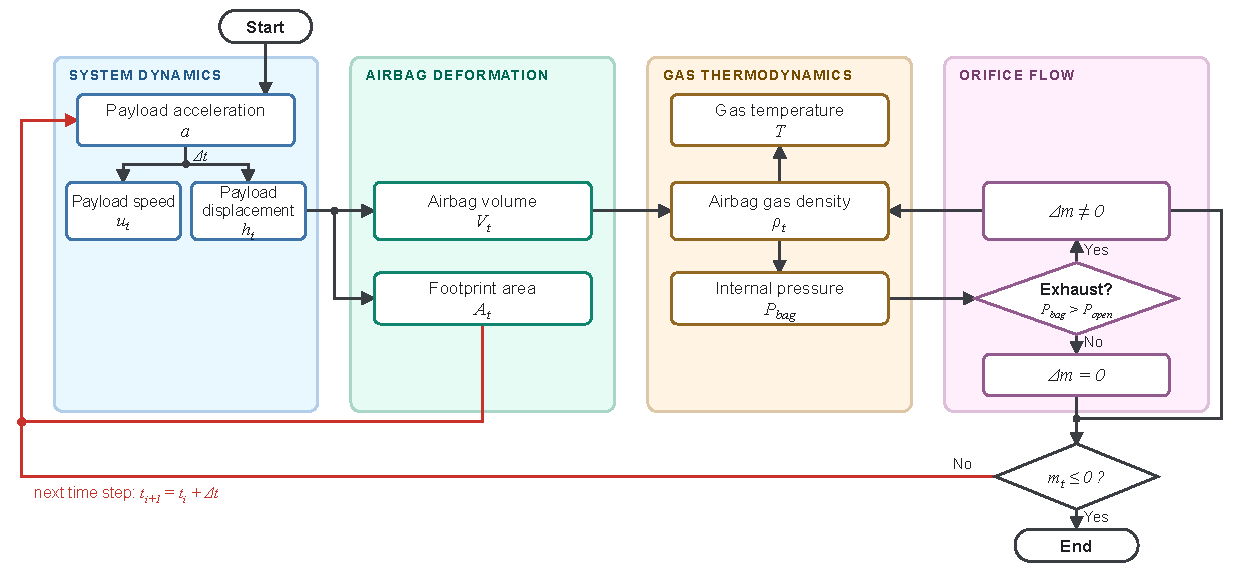
\includegraphics[width=\textwidth]{figures/chap2/Zhou-et-al_2019_flowChart.pdf}
    \caption{\hl{manca per caso la freccia di terminazione?} Calculation flowchart of the one-degree-of-freedom airbag impact model, adapted from Zhou et al. \cite{Zhou2019}.}
    \label{fig:zhou-airbag-flowchart}
\end{figure}

Except for the initial conditions and the payload's mass, these quantities are updated iteratively at each timestep to produce characteristic outputs for airbag-governed impact events such as \textit{airbag volume}, \textit{internal pressure}, \textit{internal gas mass}, \textit{payload acceleration}, \textit{payload speed}, and \textit{payload displacement}. The logic of this calculation loop is schematized in Fig.\ref{fig:zhou-airbag-flowchart}, which is an adaptation of the original diagram presented in the paper. The calculation loop is divided into four blocks, run sequentially at each timestep:

\begin{enumerate}
  \item \textbf{System dynamics step}: The resultant acceleration $a$ acting on the payload is calculated based on the reaction force from the ground calculated in the previous time step, and then integrated using the \textit{\hl{central difference scheme NEEDS MORE DETAIL?}} to obtain payload velocity $u_t$ and displacement (or stroke) $h$.
  \item \textbf{Airbag deformation step}: The airbag volume $V_t$ and footprint area $A_t$ on the ground surface are updated according to the kinematic information from the previous timestep. In this step, the hypothesis linking the stroke to the footprint area is enforced based on geometric assumptions, as mentioned earlier.
  \item \textbf{Gas thermodynamics step}: The state variables of the gas are updated assuming adiabatic compression, as it is safe to assume that little to no heat is exchanged during the rapid compression process.
  \item \textbf{Orifice flow step}: This critical step accounts for energy dissipation during the impact event. By modelling the outward airflow as flow through a one-way valve, treated as an orifice embedded in an impermeable fabric, typical nozzle fluid dynamics equations are applied to calculate the $\Delta m$ vented at each timestep. In the case of this specific paper, mass is vented only if the internal pressure $P_{bag}$ exceeds threshold pressure $P_{open}$, greater than atmospheric pressure $P_{amb}$. Within a single timestep, venting takes place as long as the exhaust condition withstands, updating gas density $\rho_t$ and recalculating the gas' temperature $T$ and pressure in an internal feedback loop. 
\end{enumerate}

In \cite{Zhou2019}'s framing, the code stops either when the manually-set duration of the phenomenon is reached, or when all mass is vented off. Testing of the code indicates that the no-rebound condition shown in the paper is numerically enforced by introducing an if-check managing the application of the reaction force.

The core work of the present thesis resides in turning the working principle of airbag impact events as presented in \cite{Zhou2019} into an informed, multi-variable problem that requires numerical optimisation. The code presented in later Section \ref{section:optimisation-code} is an expanded version of this implementation, incorporating additional criteria and alternative termination mechanisms.


\subsection{Design guidelines, requirements, and variables}\label{section:airbag-design-guidelines}
\subsubsection{Framing}
In essence, an airbag can be considered as an energy absorber and dissipator that must bring the payload from its impact velocity $v$ to rest within an available stroke $h$, without exceeding an allowable deceleration $a$. This relation is expressed in its most basic form by the kinematic relation \cite{Smith2007,Crane1985}
\begin{equation}
    h = \frac{v^2}{2a}
    \label{eq:basic-stroke-calc}
\end{equation}
which shows the central trade-off in airbag design: the lower the allowable deceleration, the longer the stroke needed to decelerate the payload and, therefore, the larger the airbag. During compression, the airbag behaves as a non-linear spring whose stiffness depends on its geometry and venting characteristics \cite{DoDeWeck2012,Zhou2019,Cole1993}. Venting is what dissipates the absorbed energy \cite{DoDeWeck2012}; whatever energy remains stored in the gas at the end of the stroke is returned to the payload as rebound \cite{WarrickLee2001}. Increasing the volume of the airbag and inflation pressure raises its energy dissipation capacity, but at the cost of higher membrane loads on the fabric \cite{Smith2007,DoDeWeck2012}.

\subsubsection{Configuration concepts}
Airbags are generally classified into three types depending on whether they contemplate the presence of venting in their design: \textit{non-vented}, \textit{vented}, and \textit{combined} \cite{Zhou2019}. A combined airbag usually consists of an outer, main-venting airbag and an inner, non-venting, anti-bottoming airbag. This "bag within a bag" concept prevents the payload from bottoming out once the outer bag has vented \cite{DoDeWeck2012,Tutt2008,GardinierTaylor1999}, and commonly relies on complex sequential inflation of the outer and inner bags \cite{GardinierTaylor1999}. An alternative to this design is using multiple airbags side by side rather than one within the other, following a "fail-safe" design philosophy by sharing impact loads and providing redundancy in case of airbag failure \cite{Smith2007}. Rather than completely enveloping the payload, the airbag can act as a buffer cushion beneath it \cite{GardinierTaylor1999}, or inflate between plates attached to the sides of the cargo \cite{Taylor2001}. Moreover, venting can be passive, activated pneumatically, or active, activated electronically \cite{WarrickLee2001,HolnickiSzulc2009}. Active venting is the basis of adaptive impact absorption, in which the airbag responds to the actual, case-specific impact load \cite{HolnickiSzulc2023}: for example, in multi-chamber designs, controllable valves allow gas to flow between adjacent chambers and to the environment, redistributing a non-uniform load across the structure \cite{HolnickiSzulc2009,HolnickiSzulc2015}.

\subsubsection{Design requirements}
Notable airbag design requirements and recommendations identified in literature are summarised in Table \ref{tab:requirements} and relate to impact conditions, such as the vertical and horizontal velocity, impact attitude, and landing surface \cite{McCullough1964,Smith2007,DoDeWeck2012}; to the allowable deceleration of the payload; and to general constraints on mass, packaging volume and deployment time \cite{HolnickiSzulc2023,GardinierTaylor1999,Cadogan2002}.

% requirements table
{\longtablesetup
\begin{longtable}{G{0.19} L{0.51} L{0.30}}
\caption{Design requirements for airbag landing and impact-attenuation systems identified in the literature.}
\label{tab:requirements}\\
\headrow\hd{Category} & \hd{Requirement} & \hd{Sources} \\
\endfirsthead
\headrow\hd{Category} & \hd{Requirement} & \hd{Sources} \\
\endhead
\contfoot{3}
\endfoot
\lastrule
\endlastfoot

% ---------------------------------------------------------------------
Dynamics
& Limit the peak acceleration transmitted to the payload & \cite{HolnickiSzulc2023,GardinierTaylor1999,Lim2015,DoDeWeck2012,Alekseychuk2024} \\
\itemrule{2}
& Reduce the touchdown velocity to a target value & \cite{HolnickiSzulc2023} \\
\itemrule{2}
& Cope with horizontal velocity (non-nominal impact attitudes coupling) & \cite{Smith2007,DoDeWeck2012,McCullough1964} \\
\grouprule
% ---------------------------------------------------------------------
Landing conditions
& Cope with different landing surfaces & \cite{McCullough1964,Shen2025,Tutt2008} \\
\itemrule{2}
& Avoid fabric rupture and tearing & \cite{DoDeWeck2012,Cadogan2002} \\
\itemrule{2}
& Prevent bottoming-out of the payload & \cite{GardinierTaylor1999,DoDeWeck2012,Tutt2008,Zhou2019} \\
\itemrule{2}
& Limit rebound and prevent rollover & \cite{WarrickLee2001,GardinierTaylor1999} \\
\grouprule
% ---------------------------------------------------------------------
Inflation pre-landing
& Synchronise venting and payload contact & \cite{CasidayFrey2000} \\
\itemrule{2}
& Deploy fully within the available time & \cite{HolnickiSzulc2023,GardinierTaylor1999} \\
\itemrule{2}
& Retain pressure for the required duration & \cite{GardinierTaylor1999,Cadogan2002} \\
\grouprule
% ---------------------------------------------------------------------
Packaging
& Survive long-term stowage in the packed state & \cite{Cadogan2002} \\
\itemrule{2}
& Integrate with the host vehicle without interference & \cite{HolnickiSzulc2023} \\
\itemrule{2}
& Withstand the environmental temperature range & \cite{Cadogan2002,McCullough1964} \\
\grouprule
% ---------------------------------------------------------------------
General
& Minimise system mass & \cite{HolnickiSzulc2023,GardinierTaylor1999,Cadogan2002} \\
\itemrule{2}
& Allow reuse & \cite{GardinierTaylor1999,McCullough1964} \\
\itemrule{2}
& Provide redundancy against single-bag failure & \cite{Smith2007} \\
\end{longtable}
}


\subsubsection{Design variables}
All airbag design variables found in the literature analysed for the present review can be found in Table \ref{tab:variable_inventory}. The variables in the table are divided into two umbrella categories: \textit{Energy absorption at impact} and \textit{Deployment and packaging}. These categories can be mapped almost directly onto two distinct impact phases (at-impact and pre-impact behaviour, respectively) and, consequently, into two separate, although not entirely uncoupled, design stages: \textit{phase 1}, focusing on the inflated configuration during impact to \textit{limit peak acceleration} below the allowable limit set by the payload's integrity requirement, and \textit{Phase 2}, focusing on the pre-impact inflation process by mostly \textit{optimising out-of-stowage deployment time} and leading to prototyping.

% mega long table
{\longtablesetup
\begin{longtable}{G{0.13} L{0.17} L{0.46} L{0.24}}
\caption{Airbag design variables identified in the literature, grouped by design focus and subcategory, with the associated trade-offs.}
\label{tab:variable_inventory}\\
\headrow\hd{Group} & \hd{Variable} & \hd{Trade-off} & \hd{Sources} \\
\endfirsthead
\headrow\hd{Group} & \hd{Variable} & \hd{Trade-off} & \hd{Sources} \\
\endhead
\contfoot{4}
\endfoot
\lastrule
\endlastfoot

% ---------------- GROUP 1 (blue = Phase 1)
\grouphead{4}{phaseA}{Energy absorption at impact}
Geometry
  & Shape & Pressure-vessel shapes carry membrane loads well; faceted shapes are easier to build & \cite{Zhou2019,Smith2007,Tutt2008,TaylorGardinier1999,DoDeWeck2012,Shen2025} \\
\itemrule{3}
& Characteristic size & More volume absorbs more energy but raises membrane loads, chance of rebound, and overall structural weight & \cite{Smith2007,DoDeWeck2012,WarrickLee2001,Peng2021} \\
\itemrule{3}
& Payload contact area & Larger contact spreads the load; wrapping the entire payload wastes material and increases weight & \cite{Tutt2008,GardinierTaylor1999,TaylorGardinier1999} \\
\itemrule{3}
& Number of chambers & Inner anti-bottoming and multiple bags add margin and redundancy (fail-safe philosophy), but increase weight and complexity & \cite{Zhou2019,DoDeWeck2012,Tutt2008,GardinierTaylor1999,Smith2007,HolnickiSzulc2009} \\
\itemrule{3}
& Tethers and webbing & Divert inertial loads from the fabric and control the shape, at the cost of added parts & \cite{Shen2025,Tutt2008,Tutt2009} \\
\grouprule
Fabric
  & Fabric type & Strength, tear resistance, low permeability, temperature flexibility vs.\ mass, packability & \cite{Cadogan2002,Tutt2008,Tutt2009,GardinierTaylor1999,Shen2025,Verma2025,Alekseychuk2024,CasidayFrey2000,Hirth2007,Lee2009,Dobrich2014} \\
\itemrule{3}
& Fabric thickness & Thicker fabric raises the rupture margin but slows deployment, enlarges the package, and increases weight & \cite{Yang2015,Lim2015,DoDeWeck2012} \\
\grouprule
Venting
  & Vent area & Larger orifices dissipate more energy and limit rebound, but risk bottoming-out & \cite{Smith2007,DoDeWeck2012,Cole1993} \\
\itemrule{3}
& Vent location & Sets the outflow and whether the ground or payload blocks the vent during the stroke & \cite{Tutt2008} \\
\itemrule{3}
& Vent burst pressure & Early opening lowers the peak pressure and resultant acceleration but spends stroke; late opening raises the peak pressure and acceleration & \cite{Smith2007,CasidayFrey2000} \\
\itemrule{3}
& Fabric porosity & Distributed gas leakage dissipates energy without vents but reduces pressure retention & \cite{Yang2015,Lim2015,KhanMoatamedi2008,Fokin2003,Cadogan2002} \\
\itemrule{3}
& Vent actuation & Active valves adapt to the actual impact; passive valves need no sensing or power & \cite{WarrickLee2001,HolnickiSzulc2009,HolnickiSzulc2015,HolnickiSzulc2023,Tutt2008,GardinierTaylor1999} \\
\grouprule
Gas
  & Initial bag pressure & Higher pressure stops the payload in a shorter stroke but raises membrane loads & \cite{Smith2007,DoDeWeck2012,CasidayFrey2000} \\
\itemrule{3}
& Gas composition & Specific-heat ratio sets compression stiffness; mixtures cut temperature sensitivity & \cite{CasidayFrey2000,Jang2021,Alekseychuk2024,Verma2025,Tutt2008} \\
% ---------------- GROUP 2 (teal = Phase 2)
\grouphead{4}{phaseB}{Deployment and packaging}
\tintB Inflation
  & Inflator type & Pyrotechnic vs.\ stored compressed gas: drives gas output, package size and triggering mechanism & \cite{Verma2025,Madlung1996,CasidayFrey2000,Jang2021,Tutt2008} \\
\itemruleB{3}
\tintB & Inflator supply pressure & Faster filling vs.\ higher deployment loads; the flow chokes at sonic conditions & \cite{KhanMoatamedi2008,CasidayFrey2000} \\
\itemruleB{3}
\tintB & Inflator mass flow rate & Shorter injection time vs.\ higher deployment loads & \cite{Yang2015,Lim2015,KhanMoatamedi2008} \\
\itemruleB{3}
\tintB & Inflator gas temperature & More pressure per unit gas mass vs.\ thermal load on the fabric just after inflation & \cite{Yang2015,Lim2015,Tutt2008,Cadogan2002} \\
\groupruleB
\tintB Housing
  & Housing size and geometry & Compact housings save mass and volume but pack the bag tighter & \cite{Munoz2007,Lim2015} \\
\itemruleB{3}
\tintB & Housing material & Plastic saves mass over metal; metal bases give a stiff mounting & \cite{Crane1985,Munoz2007,Verma2025,Lim2015} \\
\groupruleB
\tintB Folding
  & Folding pattern & Governs unfolding kinematics, deployment time and pre-stress in the packed fabric & \cite{Lee2009,Munoz2007,Ruff2007,Kamiji1998,Yang2015,Ritmeijer2005,KhanMoatamedi2008,Thornton2004,Cadogan2002} \\
\itemruleB{3}
\tintB & Number of folds & Smaller package vs.\ longer, less predictable unfolding & \hl{RIVEDI LIBRI DI MATEMATICA DELLA CERAGIOLI} \\
\groupruleB
\tintB Seams
  & Seam locations & Seams concentrate stress and are the main failure site; patterning minimises their number & \cite{Cadogan2002,Tutt2009,Bulathsinghala2021} \\
\end{longtable}
}

The table conveys the complexity of the design problem at hand, highlighting the large number of design variables. Multi-variable problems typically require an optimisation process where an optimal combination of variable values is achieved through guided iterations based on penalty concepts. This consideration forms the basis for the following chapters, in which the airbag design process is distilled into an ad-hoc workflow tailored for a specific payload application and impact scenario, focusing on a single design phase among the two presented. It is now possible to define the research-development objectives of the present thesis, leading to the proposed solution in Chapter \ref{chapter:methodology} and the specific implementation choices presented in Chapter \ref{chapter:results}.


\section{Research-Development Objective}

Having presented the context in which the research project is allocated and having gathered the necessary design information, it is possible to address the requirements set by the project commissioners:
\begin{itemize}
    \item Identify and characterise the mechanical allowables of typical medical payloads based on general packaging requirements for UAV-transported medical goods;
    \item Develop an informed conceptual design of an airbag system capable of deploying during emergency release conditions to absorb impact energy and preserve payload integrity.
\end{itemize}

These requirements can be summarised in the following Research-Development Objective and Research Questions:

\begin{objectivebox}{Research-Development Objective}
Develop and validate a design workflow to model and simulate an airbag-based protective system for UAV medical payloads using LS-DYNA, with the primary objective to ensure the structural integrity of pharmaceutical materials and their containment during drone failure and emergency payload release, thereby preventing environmental dispersion and supporting certification requirements.
\end{objectivebox}

\begin{objectivebox}{Research Question(s)}
How can a systematic multi-phase simulation workflow be developed to design an airbag-based protective system for medical payloads during UAV emergency-release events?

\textbf{Sub-questions:}
\begin{enumerate}
    \item What are the allowable mechanical limits (acceleration, stress, etc.) for medical products during emergency release, and how should these define the design envelope?
    \item How can the inflated airbag configuration be optimised to satisfy impact-absorption requirements while balancing competing design requirements?
    \item What recommendations facilitate transforming the inflated geometry into a compact, functional deployment system?
\end{enumerate}
\end{objectivebox}
